\chapter{New Material LMS Backprop}
\chapterauthor{Jeff Yoshimi}

\subsection{Derivation of the LMS rule}

All this can be shown using calculus. It's kind of amazing to turn the crank on the calculus, and see how it all works out giving us the rule above, with all the intuitive meaning. Run through the calculus, and we get our rule, which we saw above makes sense!

Conceptually, we are using the derivative of the error space. Since it's multi-dimensional, we call the derivative a gradient in this case. The gradient is a vector that points in the direction of change. 

We want to change the weight so that error is reduced. Let's leave the bias out for now. Then we are taking the  derivative of this error function:

\begin{eqnarray*}
E = (t - a_2)^2  =  (t - ( a_1 w_{1,2} + b_2))^2  =  (t -  a_1 w_{1,2} -  b_2)^2 
\end{eqnarray*}
with respect to a weight $w_{1,2}$.   Using the chain rule (derivative of the outside part applied to the inside part, times the derivative of the inside part), and substituting, we get

\begin{eqnarray*}
\frac{dE}{dw_{1,2}} = 2 (t - a_1 w_{1,2} - b_2) (-a_1) =  -2 a_1 (t - a_1 w_{1,2} - b_2) =  -2 a_1 (t - a_2)
\end{eqnarray*}

And since $t -  a_2$ is error $e_2$ we get

\begin{eqnarray*}
\frac{dE}{dw_{1,2}} = -2 e_2 a_1
\end{eqnarray*}

This says that the change in error with respect to the weight is given by error times source activation times a constant. The 2 can be ignored, since we can think of it as being absorbed into the learning rate. Also, this gradient points in the direction of error increasing. But we want to go in the opposite direction, so that error is reduced. So we multiply this gradient by $-1$, changing its sign. And so our learning rule is 

\begin{eqnarray*}
\Delta w_{1,2}  =  \epsilon a_1 e_2  = \epsilon a_1 (t - a_2)
\end{eqnarray*} 

Of course this generalizes, and so our general learning rule for weights is:
\begin{eqnarray*}
\Delta w_{i,j}  =  \epsilon a_i (t_j - a_j)
\end{eqnarray*} 

As an exercise, try deriving the rule for bias.  Again the error function is

\begin{eqnarray*}
E =  (t - ( a_1 w_{1,2} + b_2))^2 
\end{eqnarray*}
but in this case we want to find $\frac{dE}{db_{2}}$.

Now let's add in the activation function $f$ and derive the weight-update rule. Now the error function is:

\begin{eqnarray*}
E =  (t - f(a_1w_{1,2} + b_2))^2   
\end{eqnarray*}

and so

\begin{eqnarray*}
\frac{dE}{dw_{1,2}} = 2 (t - f(a_1w_{1,2} + b_2)) f'(a_1w_{1,2} + b_2) a_1 
\end{eqnarray*}

Subbing in $a_2 = f(a_1w_{1,2} + b_2))$, and recalling $n_2 = w_{1,2} + b_2$  and $t - a_2 = e_2$ 

\begin{eqnarray*}
\frac{dE}{dw_{1,2}}  = 2 e_2 f'(n_2) a_1 
\end{eqnarray*}

So the learning rule for weights is:
\begin{eqnarray*}
\Delta w_{i,j}  =  \epsilon a_i e_j f'(n_j)
\end{eqnarray*} 

This is the same as before, but multiplied by the derivative of the activation function applied to to the net input (the weighted input to the node). We discuss this more below. 

Note that the derivative of the activation function $f'$ is like a free parameter in this formula. Whatever your activation function $f$ is, to use gradient descent we just plug in $f'$ and we can do gradient descent. Situations like this allow backprop to be automated in a sense. BUT some derivatives have problems, like being undefined or 0, which effectively turns off update.

Intuitively, the idea is to scale the rate of weight change by how much the activation function is changing things. So when the activation function is changing things a lot, we want the weight to change a lot too. When it changes things very little, the derivative is small and so we change the weight less.  It doesn't matter as much.  Also note that if the derivative is 0, then learning stops. That can be a problem with piecewise linear and relu activation functions, and is why the threshold activation function can't be used at all.  Again see below.

\section{Vector approach to LMS}

% TODO: Write some new material just for the new representation

In the scalar approach to LMS we multiply a single output error (target - output) by source activation. Now we have a vector of errors times a vector of source activations. But how to deal with indexing?  The algorithm is ultimately a variant on Hebb, so we already have a template for thinking about it.

The error part itself is easy, first we do target - output using elementwise subtraction: $\mathbf{t} - \mathbf{a}_{\text{out}}$.  To multiply these errors times source activations, we do the same thing as in Hebb: we multiply an $m \times  1$ column output errors times a $1 \times  n$ row of source activations to get an $m \times n$ matrix of weight deltas.  Then we scale that by learning rate, and add to the weight matrix.  (There remains the issue of the bias, and any activation functions on the output, but we're starting simple.) So, the vectorized rule is
\begin{eqnarray*}
\Delta \mathbf{w}  =  \epsilon (\mathbf{t} - \mathbf{a}_{\text{out}}) \mathbf{a}_{\text{in}}^T
\end{eqnarray*}
Remember, by default all vectors in bold face are column vectors.  So this is a column vector (the error $\mathbf{t} - \mathbf{a}_{\text{out}}$) times a row vector (the input activations) which produces a matrix in the same shape as the weight matrix.

Consider the network shown in figure \ref{lms_vector_pre}.

\begin{figure}[h]
\centering
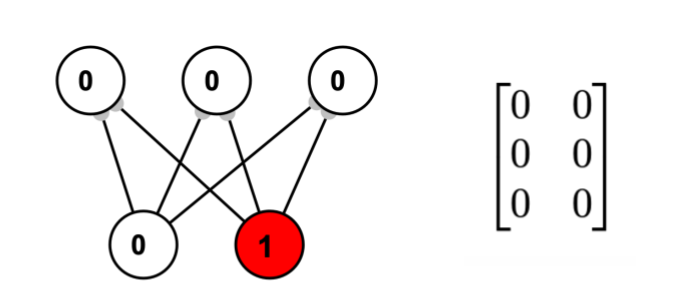
\includegraphics[width=0.55\textwidth]{images/vectorLMSBeforeTrain.png}
\caption[Jeff Yoshimi.]{A network with empty weights. We want it to learn to associate $(0,1)$ input to $(1,0,1)$}
\label{lms_vector_pre}
\end{figure}

Remember, the weight matrix is a 3x2 matrix  (``target-source''), which we are treating as all zero in this example. Each row is a fan-in of an output node, and the columns are fan-outs of input nodes. Our template for thinking about this is to imagine inputs coming up from the bottom, and dotting with the fan-in weight vectors to produce outputs (really net-inputs, to which bias is added and an activation function applied)

Our values are
\begin{equation*}
\epsilon = 1 \; \; \\
\mathbf{a}_{\text{in}} = \begin{bmatrix} 0 \\ 1 \end{bmatrix} \\
\mathbf{t} = \begin{bmatrix} 1 \\ 0 \\ 1 \end{bmatrix}
\mathbf{a}_{\text{out}} = \begin{bmatrix} 0 \\ 0 \\ 0 \end{bmatrix}
\end{equation*}

Then the equation is learning rate times error times input transposed:

\begin{align*}
\Delta \mathbf{w}  = 1
\begin{bmatrix} 1 \\ 0 \\ 1 \end{bmatrix} 
\begin{bmatrix} 0 & 1 \end{bmatrix} 
= \begin{bmatrix} 1 \cdot 0 & 1 \cdot 1 \\ 0 \cdot 0 & 0 \cdot 1 \\ 1 \cdot 0 & 1 \cdot 1 \end{bmatrix} 
= \begin{bmatrix} 0 & 1 \\ 0 & 0 \\  0 & 1  \end{bmatrix}
\end{align*}

So we get

\begin{align*}
\mathbf{w} + \Delta \mathbf{w}  =
\begin{bmatrix} 0 & 0 \\ 0 & 0 \\  0  & 0  \end{bmatrix} +
\begin{bmatrix} 0 & 1 \\ 0 & 0 \\  0  & 1  \end{bmatrix} =
\begin{bmatrix} 0 & 1 \\ 0 & 0 \\  0  & 1  \end{bmatrix}
\end{align*}

And again, keeping in mind that rows are fan-in of output and columns are fan-out of input we get figure \ref{lms_vector_2}.

\begin{figure}[h]
\centering
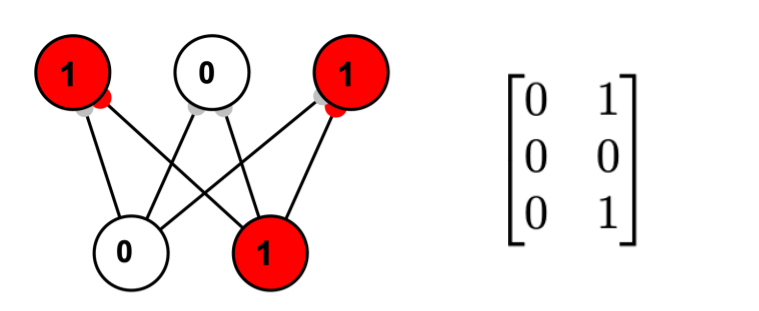
\includegraphics[width=0.55\textwidth]{images/vectorLMSAfterTrain.png}
\caption[Jeff Yoshimi.]{The network after training}
\label{lms_vector_2}
\end{figure}

We can now check that it works. Remember, think of the column vector on the right as ``entering'' from below, and dotting with each fan-in weight vector (each row of the matrix) to produce the output.  SSE has gone to 0 in a single time step.

\begin{align*}
\begin{bmatrix} 0 & 1 \\ 0 & 0 \\  0  & 1  \end{bmatrix}
\begin{bmatrix} 0 \\ 1 \end{bmatrix}
= \begin{bmatrix} 1 \\ 0 \\ 1  \end{bmatrix}
\end{align*}

% Add exercizes here, use Mak and David examples.
So now I suggest you try some examples of your own.  Come up with your own training set, apply the rule and see if you can run this a few times.  

\subsection{Bias}

To add bias updates in, we just vectorize the bias update rule, which has the same form as the scalar rule, since it's just elementwise.

\begin{eqnarray*}
\Delta \mathbf{b}  =  \epsilon (\mathbf{t} - \mathbf{a}_{out})
\end{eqnarray*}

So at each iteration, we change the bias vector just in the direction of the error vector. Remember goldilocks.  When things are too hot, cool them down. Etc.

\subsection{Activation functions}

(This material can also be added to the scalar case)


The full LMS rule also involves a derivative on the activation function.  These derivatives can be understood pretty intuitively if we look at those again. See figure \ref{derivativesActFunctions}.  The derivative for the threshold function is 0 everywhere except at the threshold where it is undefined (this was a problem for Rosenblatt). The derivative for the piecewise linear is 0 above and below the upper and lower bounds and the slope (usually 1) of the function in between those bounds. For the sigmoid it's close to what it is for piecewise linear, approaching 1 as net input is large or small and the slope at the inflection point in the middle, but we do need a formula for it.

\begin{figure}[h]
\centering
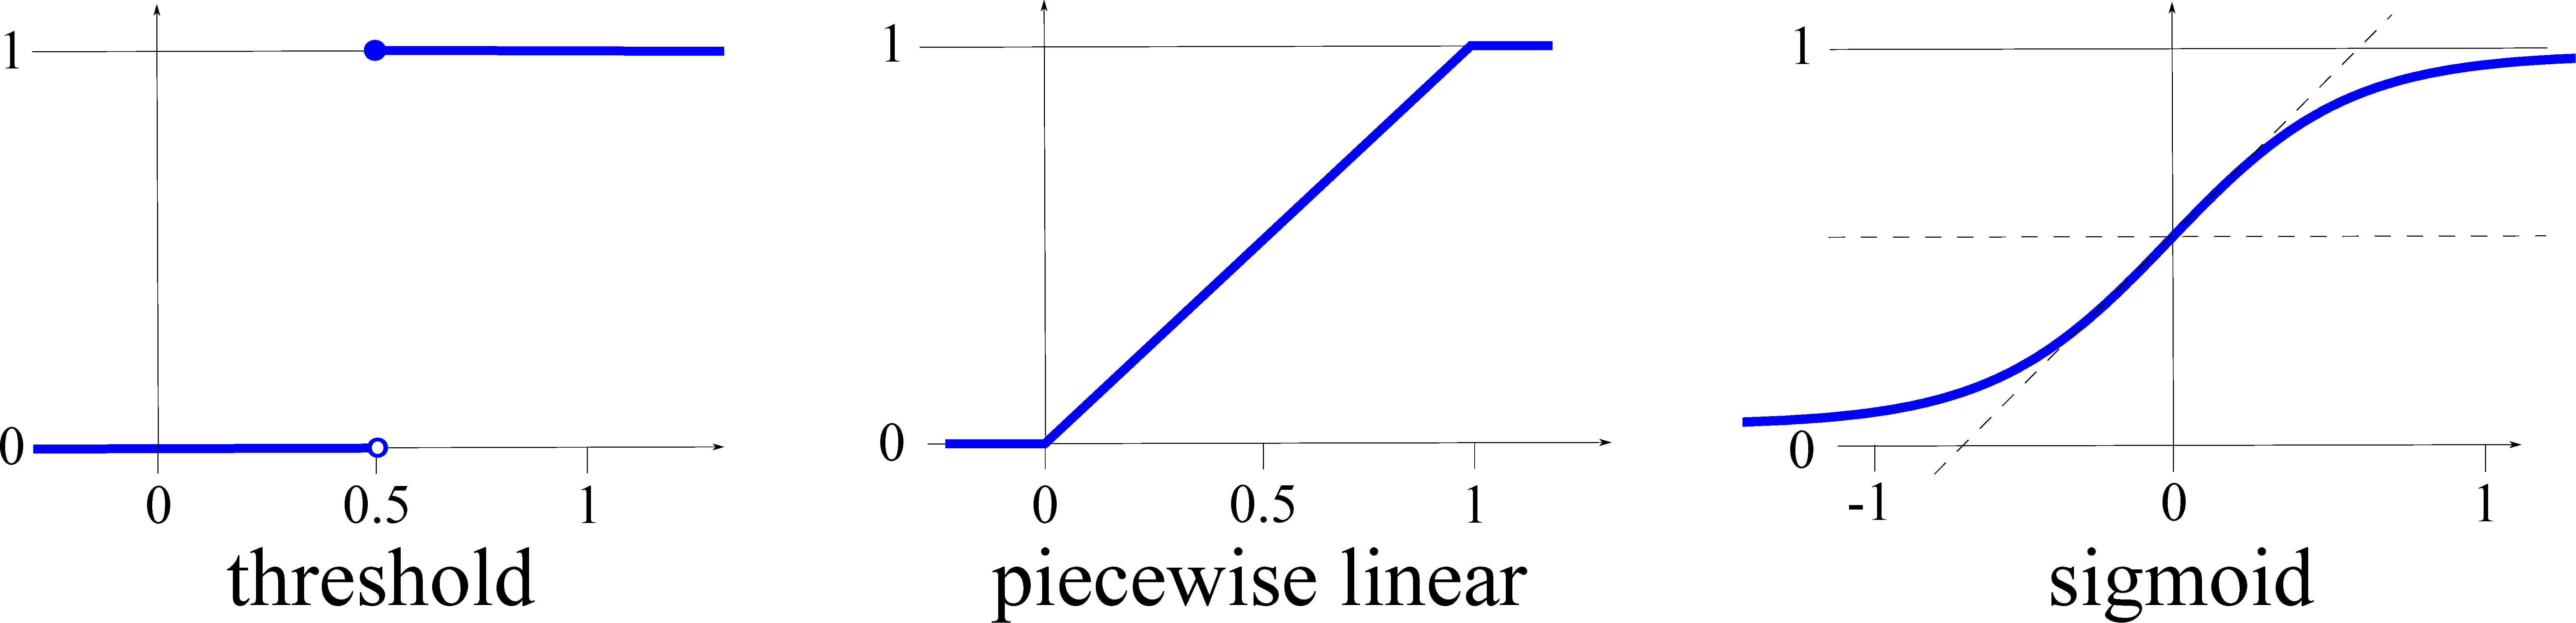
\includegraphics[width=0.75\textwidth]{images/graph_binary.pdf}
\caption[Jeff Yoshimi.]{The activation functions. The derivative is either 0 or the slope or close to the slope in most cases. }
\label{derivativesActFunctions}
\end{figure}

So how to work this into the LMS error update?

First, recall from chapter \extref{ch_act_functions} that the weighted input to a node $j$ is denoted $n_j$. This is the same as the activation of a linear unit. Its weights times input activations plus a bias.  An activation function $f$ then transformed this weighted inputs, so that $a_j = f(n_j)$.  When we incorporate activation functions we have to keep $a_j$ and $n_j$ separate so just get that clear before moving on.

Ok, and recall from the derivation that error update with an activation function involves the same as before multiplied by with the derivative of the activation function applied to to the net inpu.  Intuitively it's like we scale the error that we use to scale the weights and biases with a factor corresponding to how much the activation function changes things.\footnote{This is a problem with RELU, known as the ``dying Relu" problem.}  It's also why Rosenbatt's perception was limited; binary are 0 derivative everywhere so their weights never change using this rule, and so he had to come up with a kind of ad hoc solution.

So  the full rule for weights is

\begin{eqnarray*}
\Delta w_{i,j}  =  \epsilon a_i (t_j - a_j) f' (n_j)
\end{eqnarray*}

And the full rule for biases is 

\begin{eqnarray*}
\Delta b_{j}  =  \epsilon b_j (t_j - a_j) f' (n_j)
\end{eqnarray*}

Do both of these at each time step to update the network.

\subsection{The Full Vectorized LMS rule}

Putting it all together, thevectorized rule is

\begin{eqnarray*}
\Delta \mathbf{w}  =  \epsilon (\mathbf{t} - \mathbf{a}_{\text{out}}) f'( \mathbf{n}_{\text{out}}) \mathbf{a}_{\text{in}}^T
\end{eqnarray*}

We take a column of errors (targets - outputs), and scale each component by the derivative of the activation function applied to the weighted inputs. Remember, weighted inputs is just one more quantity that each node has. When it's updated, it must compute that, and then use that to compute the activation value. So the node has both values, and so we can easily get components of this column vector: we have the target, the output activation, and the net input at any time, and that is enough to get us the column vector. We then matrix multiply that by a row of source activations and the result is a matrix of weight deltas with the right shape.

\begin{eqnarray*}
\Delta \mathbf{b}  =  \epsilon (\mathbf{t} - \mathbf{a}_{\text{out}}) f'( \mathbf{n}_{\text{out}})
\end{eqnarray*}

All of these vector operations should be familiar. For the application of $f$, it's just a matter of apply it to each component of the vector.  For example, if $f(x) = x+1$ then $f(1,2) = (2,3)$. $f'$ is just a function so it can be applied in this way to a vector.

